\graphicspath{ {figuras/} }
\chapter[Processo de Engenharia de Requisitos]{Processo de Engenharia de Requisitos}\label{cap4}

Esse processo foi desenhado utilizando ferramenta ``\textit{BIZAGI modeler}''. Houveram 5 evoluções,
presentes no apêndice A, a partir do primeiro esboço até chegar a versão apresentada na imagem \ref{fig:processo}.

Como foi descrito no capítulo \ref{cap3} o processo criado foi estruturado baseando-se no
SAFe mantendo os três níveis estruturais do framework, portifólio, programa e time
que estão detalhados na sessão \ref{safe}.

A manutenção da rastreabilidade dos requisitos, teve papel fundamental para a criação deste processo,
uma vez que são definidos vários níveis de requisitos e o processo para manter essa
rastreabilidade no SAFe não está totalmente definido em atividades.

É fundamental destacar que o problema da escolha de um abordagem não esta em considerar
a mutabilidade dos requisitos e sim em como tratar essas mudanças que são inevitáveis.
Pensando nisso foram adicionadas atividades de gerência de mudanças baseadas no RUP,
para sanar um possível risco na comunicação e gerência do projeto devido a não experiência
de trabalho entre os membros do grupo. Esse processo ocorre de forma eventual e paralela
e será detalhado na sessão \ref{sec:gerencia}.

\begin{figure}[H]
    \centering
	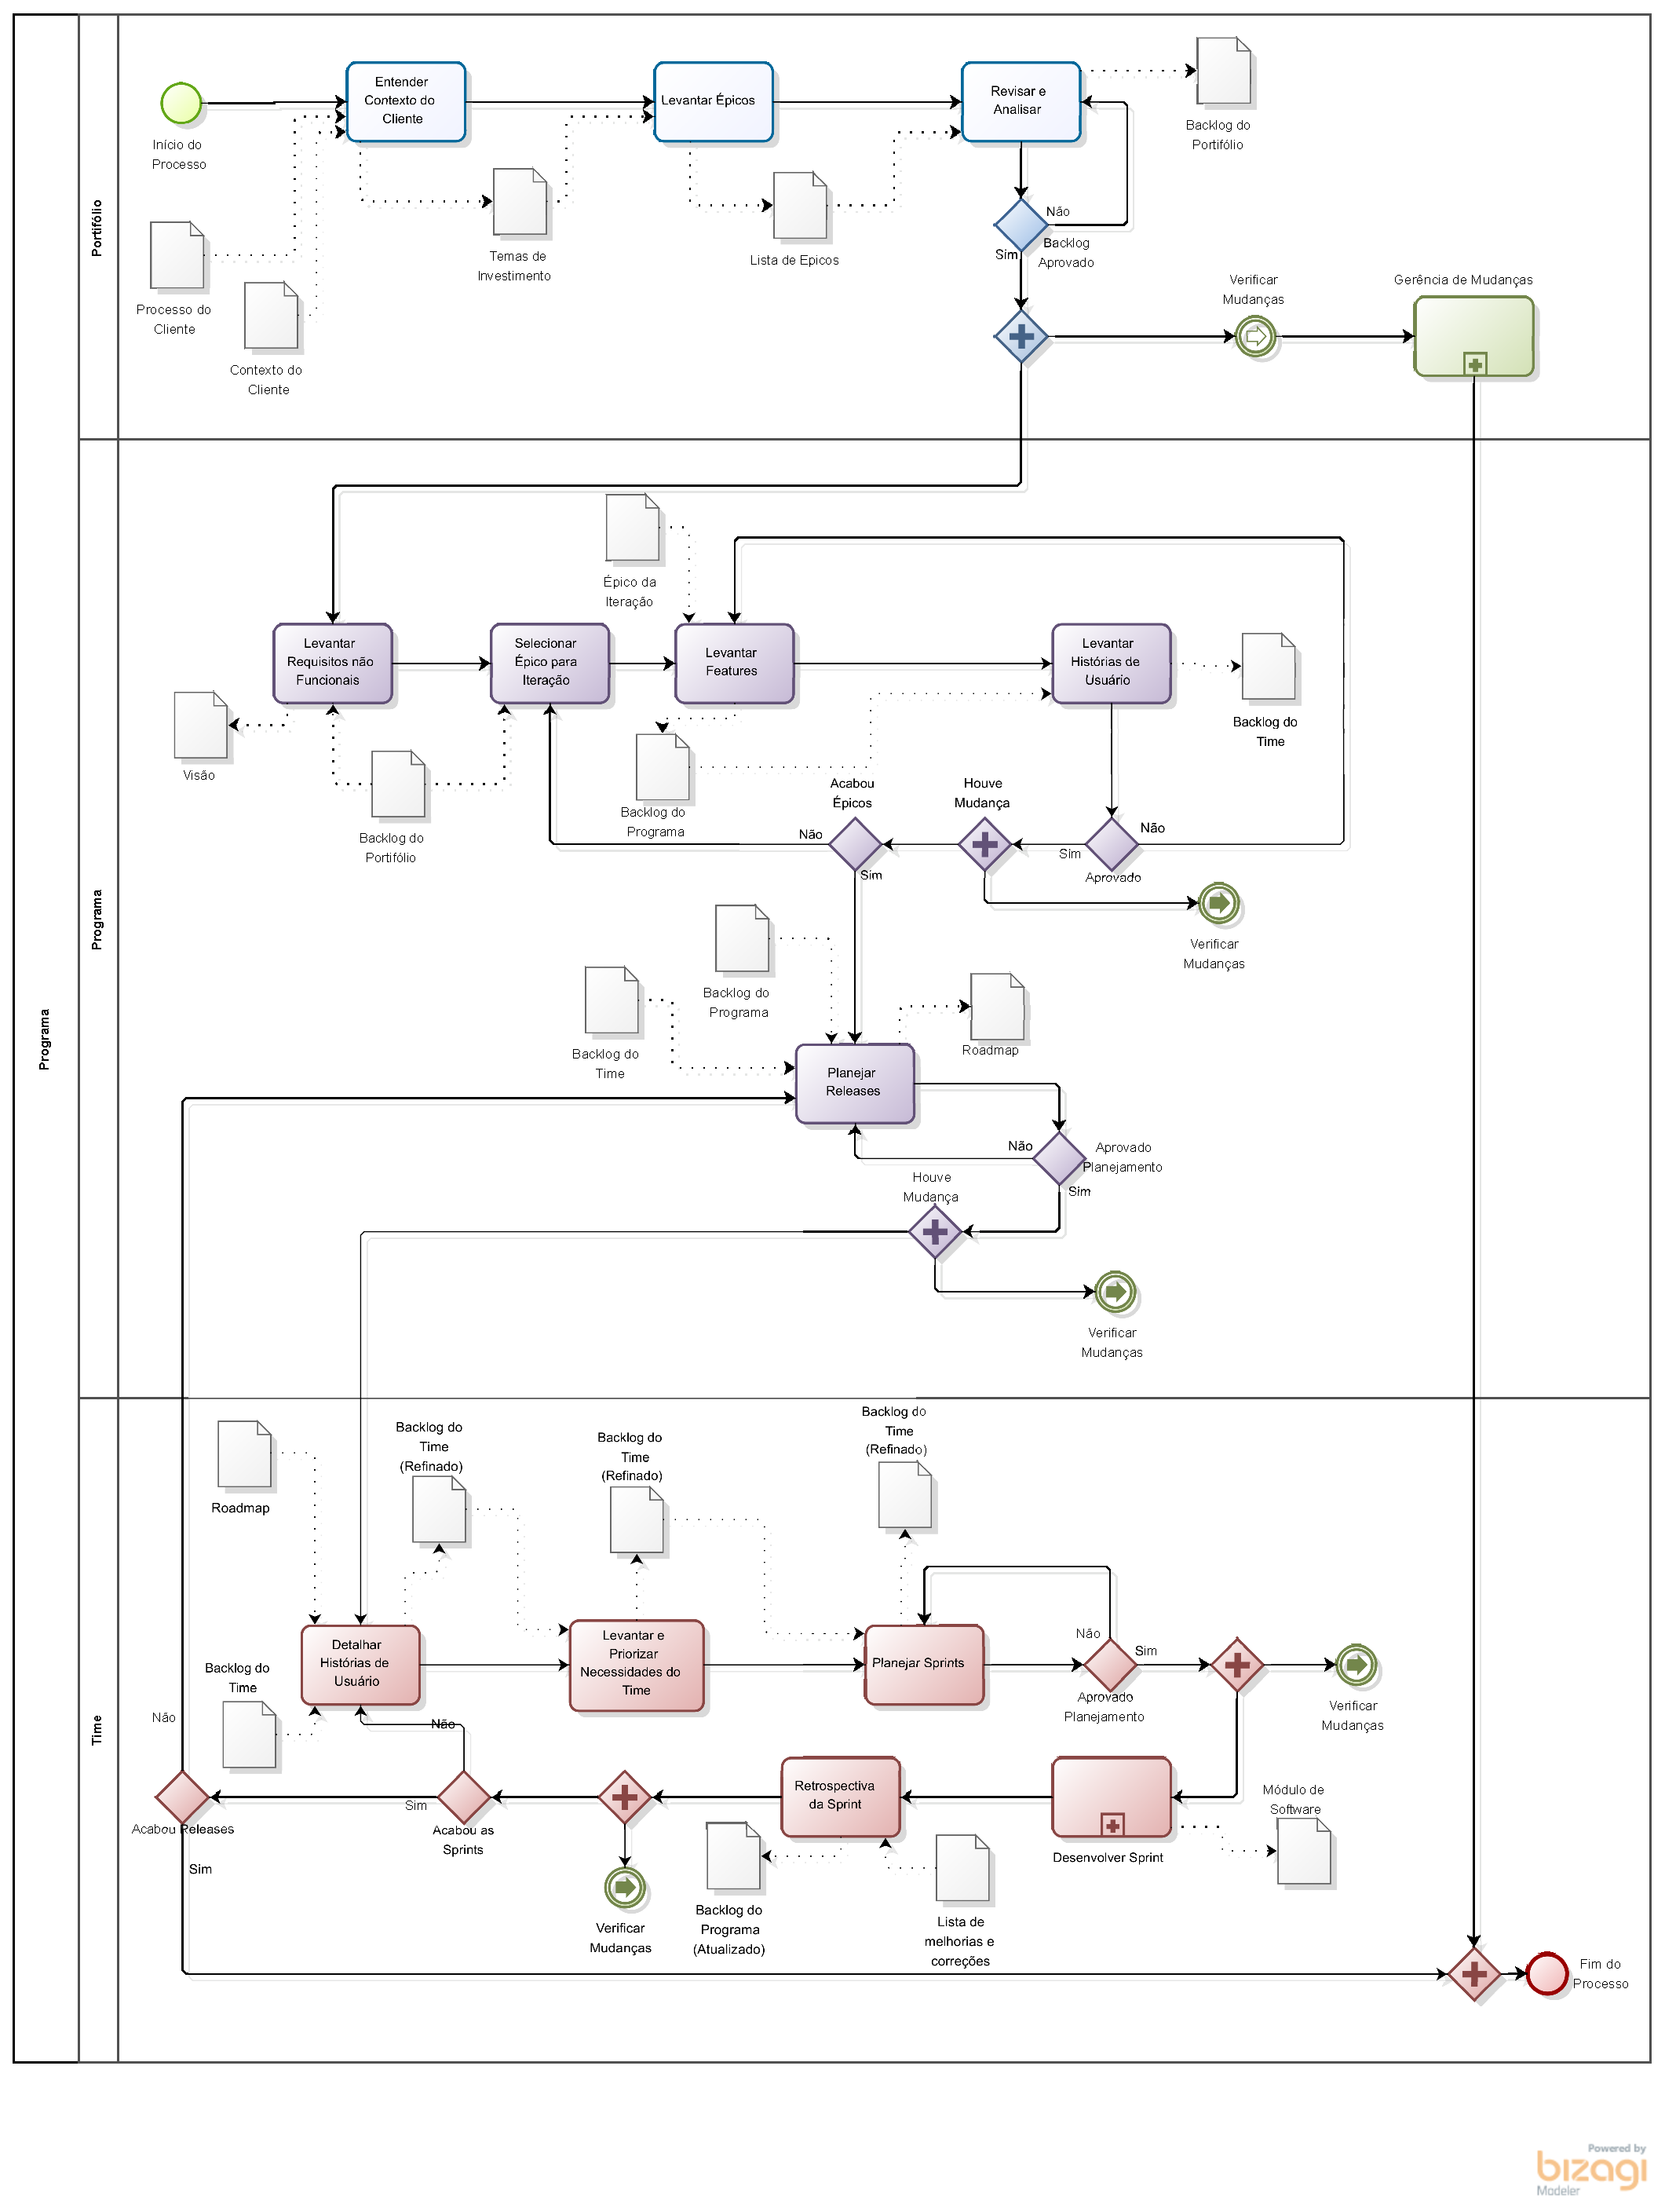
\includegraphics[keepaspectratio=true,scale=0.5]{figuras/Processo_05.eps}
    \caption{Visão geral do processo desenvolvido para o projeto.}
    \label{fig:processo}
\end{figure}

\section{Scaled Agile Framework}\label{safe}

Nessa sessão serão descritos os níveis que compoem o SAFe(Portifólio, Programa e Time).
Sendo mostrado o objetivo cada nível como também as atividades que a compoem.

\subsection{Portifólio}

No processo criado nesse trabalho, esse nível tem como objetivo levantar e estabelecer
uma abstração de alto nível dos requisitos do negócio. Esse levantamento ocorrerá
por meio da efetuação das atividades Entender Contexto do Cliente e Levantar Épicos
e Revisar e Analisar. As técnicas utilizadas para a execução de cada atividade serão
a análise documental, workshops e Brainstorms.

\subsubsection{Processo}
\subsubsection{Papéis}
\subsubsection{Artefatos}
\subsubsection{Atividades}

  \begin{table}[H]
    \centering
      \begin{tabular}{| m{5em} | m{10cm} |}
        \hline
        ID       & 01   \\ \hline
        Nome     & Entendimento do Contexto do Cliente   \\ \hline
        Objetivo & Entender o contexto de onde, para quem e o que, será desenvolvido. \\ \hline
        Entradas & Processo do Cliente e Contexto do Cliente.   \\ \hline
        Saídas   & Tema de Ivestimento. \\ \hline
        Papel Responsável   & Gerente de Portfólio. \\ \hline
      \end{tabular}
      \caption{Legenda da Tabela}
      \label{tabela:atividade1}
  \end{table}

  \begin{table}[H]
    \centering
      \begin{tabular}{| m{5em} | m{10cm} |}
        \hline
        ID       & 02   \\ \hline
        Nome     & Levantamento de épicos   \\ \hline
        Objetivo & Escrever o máximo de épicos relacionados ao tema de investimento. \\ \hline
        Entradas & Tema de Investimento   \\ \hline
        Saídas   & Épicos \\ \hline
        Papel Responsável   & Gerente de Portfólio. \\ \hline
      \end{tabular}
      \caption{Legenda da Tabela}
      \label{tabela:atividade2}
  \end{table}

  \begin{table}[H]
    \centering
      \begin{tabular}{| m{5em} | m{10cm} |}
        \hline
        ID       & 03   \\ \hline
        Nome     & Revisão e Análise   \\ \hline
        Objetivo & Revisar e Priorizar épicos. \\ \hline
        Entradas & Épicos   \\ \hline
        Saídas   & Backlog do Portifólio \\ \hline
        Papel Responsável   & Gerente de Portfólio. \\ \hline
      \end{tabular}
      \caption{Legenda da Tabela}
      \label{tabela:atividade3}
  \end{table}

  \subsection{Programa}
  \subsubsection{Processo}
  \subsubsection{Papéis}
  \subsubsection{Artefatos}
  \subsubsection{Atividades}

  \begin{table}[H]
    \centering
      \begin{tabular}{| m{5em} | m{10cm} |}
        \hline
        ID       & 04   \\ \hline
        Nome     & Levantar Requisitos não Funcionais   \\ \hline
        Objetivo & Definir RnFs. \\ \hline
        Entradas & Backlog do Portifólio   \\ \hline
        Saídas   & Visão \\ \hline
        Papel Responsável   & Gerente de Portfólio. \\ \hline
      \end{tabular}
      \caption{Legenda da Tabela}
      \label{tabela:atividade4}
  \end{table}

  \begin{table}[H]
    \centering
      \begin{tabular}{| m{5em} | m{10cm} |}
        \hline
        ID       & 05   \\ \hline
        Nome     & Selecionar Épico para Iteração   \\ \hline
        Objetivo & Selecionar o épico para a iteração de levatamento de features. \\ \hline
        Entradas & Backlog do Portifólio\\ \hline
        Saídas   & Épico da iteração \\ \hline
        Papel Responsável   & Gerente de Portfólio. \\ \hline
      \end{tabular}
      \caption{Legenda da Tabela}
      \label{tabela:atividade5}
  \end{table}

  \begin{table}[H]
    \centering
      \begin{tabular}{| m{5em} | m{10cm} |}
        \hline
        ID       & 06   \\ \hline
        Nome     & Levantar Features   \\ \hline
        Objetivo & Levantar todas a features do Épico da iteração. \\ \hline
        Entradas & Épico da Iteração\\ \hline
        Saídas   & Backlog do Programa \\ \hline
        Papel Responsável   & Gerente de Portfólio. \\ \hline
      \end{tabular}
      \caption{Legenda da Tabela}
      \label{tabela:atividade6}
  \end{table}

  \begin{table}[H]
    \centering
      \begin{tabular}{| m{5em} | m{10cm} |}
        \hline
        ID       & 07   \\ \hline
        Nome     & Levatar Histórias  \\ \hline
        Objetivo & Levantar as histórias das features que surgiram na ativade anterior.  \\ \hline
        Entradas & Backlog do Programa\\ \hline
        Saídas   & Backlog do Time \\ \hline
        Papel Responsável   & Gerente de Portfólio. \\ \hline
      \end{tabular}
      \caption{Legenda da Tabela}
      \label{tabela:atividade7}
  \end{table}

  \begin{table}[H]
    \centering
      \begin{tabular}{| m{5em} | m{10cm} |}
        \hline
        ID       & 08   \\ \hline
        Nome     & Planejar Releases  \\ \hline
        Objetivo & Planejar as releases do desenvolvimento do projeto \\ \hline
        Entradas & Backlog do Programa, Backlog do Time\\ \hline
        Saídas   & Roadmap \\ \hline
        Papel Responsável   & Gerente de Portfólio. \\ \hline
      \end{tabular}
      \caption{Legenda da Tabela}
      \label{tabela:atividade8}
  \end{table}

  \subsection{Time}
  \subsubsection{Processo}
  \subsubsection{Papéis}
  \subsubsection{Artefatos}
  \subsubsection{Atividades}

  \begin{table}[H]
    \centering
      \begin{tabular}{| m{5em} | m{10cm} |}
        \hline
        ID       & 09   \\ \hline
        Nome     & Detalhar Histórias de Usuário  \\ \hline
        Objetivo & Definir critérios para teste e aceitação da conclusão da história  \\ \hline
        Entradas & Roadmap, Backlog do Time\\ \hline
        Saídas   & Backlog do Time (Refinado) \\ \hline
        Papel Responsável   & Gerente de Portfólio. \\ \hline
      \end{tabular}
      \caption{Legenda da Tabela}
      \label{tabela:atividade9}
  \end{table}

  \begin{table}[H]
    \centering
      \begin{tabular}{| m{5em} | m{10cm} |}
        \hline
        ID       & 10   \\ \hline
        Nome     & Levantar e Priorizar Necessidades do Time  \\ \hline
        Objetivo & Entender as necessidades do time.  \\ \hline
        Entradas & Backlog do Time (Refinado)\\ \hline
        Saídas   & Backlog do Time (Refinado) \\ \hline
        Papel Responsável   & Gerente de Portfólio. \\ \hline
      \end{tabular}
      \caption{Legenda da Tabela}
      \label{tabela:atividade10}
  \end{table}

  \begin{table}[H]
    \centering
      \begin{tabular}{| m{5em} | m{10cm} |}
        \hline
        ID       & 11   \\ \hline
        Nome     & Planejar Sprints  \\ \hline
        Objetivo & Organizar Sprints necessárias para a execução da release  \\ \hline
        Entradas & Backlog do Time (Refinado)\\ \hline
        Saídas   & Backlog do Time (Refinado) \\ \hline
        Papel Responsável   & Gerente de Portfólio. \\ \hline
      \end{tabular}
      \caption{Legenda da Tabela}
      \label{tabela:atividade11}
  \end{table}

  \begin{table}[H]
    \centering
      \begin{tabular}{| m{5em} | m{10cm} |}
        \hline
        ID       & 12   \\ \hline
        Nome     & Códificar Histórias  \\ \hline
        Objetivo & ----  \\ \hline
        Entradas & Backlog do Time (Refinado)\\ \hline
        Saídas   & Candidato a versões de Software \\ \hline
        Papel Responsável   & Gerente de Portfólio. \\ \hline
      \end{tabular}
      \caption{Legenda da Tabela}
      \label{tabela:atividade12}
  \end{table}

  \begin{table}[H]
    \centering
      \begin{tabular}{| m{5em} | m{10cm} |}
        \hline
        ID       & 13   \\ \hline
        Nome     & Testar Histórias Codificada  \\ \hline
        Objetivo & ---  \\ \hline
        Entradas & Backlog do Time (Refinado)\\ \hline
        Saídas   & Versão de Software \\ \hline
        Papel Responsável   & Gerente de Portfólio. \\ \hline
      \end{tabular}
      \caption{Legenda da Tabela}
      \label{tabela:atividade13}
  \end{table}

  \begin{table}[H]
    \centering
      \begin{tabular}{| m{5em} | m{10cm} |}
        \hline
        ID       & 14   \\ \hline
        Nome     & Demonstrar Pacote de histórias desenvolvidas para o cliente. \\ \hline
        Objetivo & --- \\ \hline
        Entradas & Modulo de Software\\ \hline
        Saídas   &  --- \\ \hline
        Papel Responsável   & Gerente de Portfólio. \\ \hline
      \end{tabular}
      \caption{Legenda da Tabela}
      \label{tabela:atividade14}
  \end{table}

  \begin{table}[H]
    \centering
      \begin{tabular}{| m{5em} | m{10cm} |}
        \hline
        ID       & 15   \\ \hline
        Nome     & Coletar Melhorias e correções das histórias  \\ \hline
        Objetivo & ---  \\ \hline
        Entradas & ---\\ \hline
        Saídas   & Lista de melhorias e correções. \\ \hline
        Papel Responsável   & Gerente de Portfólio. \\ \hline
      \end{tabular}
      \caption{Legenda da Tabela}
      \label{tabela:atividade15}
  \end{table}

\subsection{Gerência de Mudança}\label{sec:gerencia}
\subsubsection{Processo}
\subsubsection{Papéis}
\subsubsection{Artefatos}
\subsubsection{Atividades}

\begin{table}[H]
  \centering
    \begin{tabular}{| m{5em} | m{10cm} |}
      \hline
      ID       & 16   \\ \hline
      Nome     & Rastrear Mudanças  \\ \hline
      Objetivo & ---  \\ \hline
      Entradas & Solicitação de Mudança\\ \hline
      Saídas   & Mudanças \\ \hline
      Papel Responsável   & Gerente de Portfólio. \\ \hline
    \end{tabular}
    \caption{Legenda da Tabela}
    \label{tabela:atividade16}
\end{table}

\begin{table}[H]
  \centering
    \begin{tabular}{| m{5em} | m{10cm} |}
      \hline
      ID       & 17   \\ \hline
      Nome     & Analisar Impacto da Mudança \\ \hline
      Objetivo & ---  \\ \hline
      Entradas & Mudanças \\ \hline
      Saídas   & Relatório de Avaliação de Mudança \\ \hline
      Papel Responsável   & Gerente de Portfólio. \\ \hline
    \end{tabular}
    \caption{Legenda da Tabela}
    \label{tabela:atividade17}
\end{table}

\begin{table}[H]
  \centering
    \begin{tabular}{| m{5em} | m{10cm} |}
      \hline
      ID       & 18   \\ \hline
      Nome     & Atualizar Backlog do Time  \\ \hline
      Objetivo & ---  \\ \hline
      Entradas & Mudanças \\ \hline
      Saídas   & Backlog do Time (Atualizado) \\ \hline
      Papel Responsável   & Gerente de Portfólio. \\ \hline
    \end{tabular}
    \caption{Legenda da Tabela}
    \label{tabela:atividade18}
\end{table}

\begin{table}[H]
  \centering
    \begin{tabular}{| m{5em} | m{10cm} |}
      \hline
      ID       & 19   \\ \hline
      Nome     & Atualizar Backlog do Programa  \\ \hline
      Objetivo & ---  \\ \hline
      Entradas & Mudanças\\ \hline
      Saídas   & Backlog do Programa (Atualizado). \\ \hline
      Papel Responsável   & Gerente de Portfólio. \\ \hline
    \end{tabular}
    \caption{Legenda da Tabela}
    \label{tabela:atividade19}
\end{table}

\begin{table}[H]
  \centering
    \begin{tabular}{| m{5em} | m{10cm} |}
      \hline
      ID       & 20   \\ \hline
      Nome     & Atualizar Backlog do Portifólio  \\ \hline
      Objetivo & ---  \\ \hline
      Entradas & Mudanças \\ \hline
      Saídas   & Backlog do Portifólio Atualizado \\ \hline
      Papel Responsável   & Gerente de Portfólio. \\ \hline
    \end{tabular}
    \caption{Legenda da Tabela}
    \label{tabela:atividade20}
\end{table}

\subsection{Desenvolvimento}
\subsubsection{Processo}
\subsubsection{Papéis}
\subsubsection{Artefatos}
\subsubsection{Atividades}
